\documentclass[aspectratio=169, 10pt]{beamer}

% --- Essential Packages ---
\usepackage[utf8]{inputenc}
\usepackage[T1]{fontenc}
\usepackage{lmodern}
\usepackage{graphicx}
\usepackage{booktabs}
\usepackage{amsmath}
\usepackage{listings}
\usepackage{tikz}
\usepackage{pgfplots}
\pgfplotsset{compat=1.18}
\usetikzlibrary{shapes,arrows,positioning,shadows,calc}

% --- Modern Styling & Colors ---
\definecolor{primary}{RGB}{20, 35, 60}     % Premium Deep Navy
\definecolor{secondary}{RGB}{0, 150, 136}   % Sleek Teal
\definecolor{accent}{RGB}{233, 30, 99}      % Coral/Pink Accent
\definecolor{darktext}{RGB}{40, 40, 40}     % Dark Charcoal for text
\definecolor{lightbg}{RGB}{248, 249, 250}   % Off-white background
\definecolor{codebg}{RGB}{244, 245, 247}    % Very light gray-blue for code

% Code syntax highlighting settings
\lstset{
    backgroundcolor=\color{codebg},
    basicstyle=\ttfamily\tiny,
    breakatwhitespace=false,
    breaklines=true,
    captionpos=b,
    commentstyle=\color{gray},
    keywordstyle=\color{primary}\bfseries,
    stringstyle=\color{accent},
    showstringspaces=false,
    frame=single,
    frameround=tttt,
    framexleftmargin=3pt,
    rulecolor=\color{primary!20}
}

% Beamer Theme Configuration
\usecolortheme{default}
\useinnertheme{rounded}
\useoutertheme{default}

% Set Beamer Colors
\setbeamercolor{palette primary}{bg=primary,fg=white}
\setbeamercolor{palette secondary}{bg=secondary,fg=white}
\setbeamercolor{structure}{fg=primary}
\setbeamercolor{background canvas}{bg=lightbg}
\setbeamercolor{normal text}{fg=darktext}
\setbeamercolor{titlelike}{bg=primary,fg=white}
\setbeamercolor{frametitle}{bg=primary,fg=white}
\setbeamercolor{block title}{bg=primary,fg=white}
\setbeamercolor{block body}{bg=white,fg=darktext}

% Custom Fonts & Typography
\setbeamerfont{title}{size=\huge,series=\bfseries}
\setbeamerfont{subtitle}{size=\large,shape=\itshape}
\setbeamerfont{frametitle}{size=\large,series=\bfseries}
\setbeamerfont{caption}{size=\scriptsize}

% Remove default navigation symbols
\setbeamertemplate{navigation symbols}{}

% Custom Header/Footer
\setbeamertemplate{headline}{}
\setbeamertemplate{footline}{
    \leavevmode%
    \hbox{%
        \begin{beamercolorbox}[wd=.333333\paperwidth,ht=2.25ex,dp=1ex,left,leftskip=3ex]{palette primary}%
            \usebeamerfont{author in head/foot}Assignment-3: Zachary
        \end{beamercolorbox}%
        \begin{beamercolorbox}[wd=.333333\paperwidth,ht=2.25ex,dp=1ex,center]{palette primary}%
            \usebeamerfont{title in head/foot}LeNet-5 \& MobileNet-V2 Evolution
        \end{beamercolorbox}%
        \begin{beamercolorbox}[wd=.333333\paperwidth,ht=2.25ex,dp=1ex,right,rightskip=3ex]{palette primary}%
            \insertframenumber{} / \inserttotalframenumber
        \end{beamercolorbox}%
    }%
    \ygap{-1pt}
}

% --- Custom TikZ Style for Diagrams ---
\tikzset{
    layer/.style={rectangle, draw=primary, fill=white, rounded corners, minimum width=2.2cm, minimum height=0.5cm, align=center, thick, drop shadow={opacity=0.1}},
    pool/.style={rectangle, draw=secondary, fill=secondary!10, rounded corners, minimum width=2.2cm, minimum height=0.5cm, align=center, thick, drop shadow={opacity=0.1}},
    fc/.style={rectangle, draw=accent, fill=accent!10, rounded corners, minimum width=2.2cm, minimum height=0.5cm, align=center, thick, drop shadow={opacity=0.1}},
    arrow/.style={thick, ->, >=stealth, draw=primary!80}
}

% --- Presentation Details ---
\title{Evolution of CNNs: LeNet-5 to MobileNet-V2}
\subtitle{Assignment-3: Deep Learning Architectures}
\author{Zachary}
\date{May 2026}

\begin{document}

% ==================== Title Slide ====================
{
\setbeamertemplate{footline}{}
\begin{frame}[plain]
    \centering
    \vspace{1.5cm}
    \begin{beamercolorbox}[sep=12pt,center,rounded=true,shadow=true]{title}
        \usebeamerfont{title}\inserttitle\par%
        \ifx\insertsubtitle\@empty%
        \else%
            \vskip0.25em%
            {\usebeamerfont{subtitle}\usebeamercolor[fg]{subtitle}\insertsubtitle\par}%
        \fi%
    \begin{tikzpicture}[remember picture, overlay]
        \draw[secondary, line width=4pt] (-6,-2.2) -- (6,-2.2);
    \end{tikzpicture}
    \end{beamercolorbox}%
    \vskip1em\par
    \begin{beamercolorbox}[sep=8pt,center]{author}
        \usebeamerfont{author}\insertauthor\\
        \small Course: Deep Learning (CNNs) -- Individual Assignment
    \end{beamercolorbox}
    \begin{beamercolorbox}[sep=8pt,center]{date}
        \usebeamerfont{date}\insertdate
    \end{beamercolorbox}
    \vspace{0.5cm}
\end{frame}
}

% ==================== Agenda ====================
\begin{frame}{Assignment Objectives \& Agenda}
    \begin{columns}
        \begin{column}{0.5\textwidth}
            \textbf{Assignment Objectives:}
            \begin{itemize}
                \item Understand the evolution of CNN architectures.
                \item Study predecessors & architectural innovations.
                \item Evaluate models on realistic datasets (MNIST & Face Anti-Spoofing).
                \item Analyze strengths, weaknesses, & computational trade-offs.
            \end{itemize}
        \end{column}
        \begin{column}{0.5\textwidth}
            \textbf{Presentation Outline:}
            \begin{enumerate}
                \item \textbf{Evolutionary Context} (Classical vs. Modern Deep CNNs)
                \item \textbf{LeNet-5} (Predecessor, Innovations, Annotated Keras Code & Evaluation)
                \item \textbf{MobileNet-V2} (Evolution from V1, Bottlenecks, Annotated Code & Performance Evaluation)
                \item \textbf{Comparative Trade-off Analysis}
            \end{enumerate}
        \end{column}
    \end{columns}
\end{frame}

% ==================== The CNN Evolutionary Paradigm ====================
\begin{frame}{The CNN Evolutionary Paradigm (1998 -- 2018)}
    \centering
    \begin{tikzpicture}[node distance=1.5cm, auto, scale=0.75, every node/.style={transform shape}]
        % Timeline blocks
        \node (lenet) [layer, fill=primary, text=white] {\textbf{LeNet-5 (1998)}\\61K Params\\Input: 32x32x1\\Focus: Digit Recognition};
        \node (alexnet) [layer, right=1.5cm of lenet] {\textbf{AlexNet (2012)}\\60M Params\\GPU Training, ReLU, Dropout\\Focus: ImageNet Scale};
        \node (resnet) [layer, below=1.0cm of alexnet] {\textbf{ResNet (2015)}\\25M+ Params\\Residual/Skip Connections\\Focus: Overcoming Gradient Vanishing};
        \node (mobilenet) [layer, fill=secondary, text=white, left=1.5cm of resnet] {\textbf{MobileNet-V2 (2018)}\\2.2M+ Params\\Inverted Residuals & Bottlenecks\\Focus: Mobile Efficiency};

        \draw [arrow] (lenet) -- (alexnet);
        \draw [arrow] (alexnet) -- (resnet);
        \draw [arrow] (resnet) -- (mobilenet);
    \end{tikzpicture}
    \vspace{0.3cm}
    \begin{itemize}
        \item \textbf{Pre-1998:} Fully Connected (Dense) networks dominated. Extremely high weights, loss of spatial structure, translation-sensitive.
        \item \textbf{1998 -- 2015:} Massive scaling in depth and parameters. Heavy GPU reliance.
        \item \textbf{Post-2015:} Pivot from purely ``deeper'' networks to ``smarter'' blocks (Residuals, separable convolutions) to maximize efficiency and portability on edge devices.
    \end{itemize}
\end{frame}

% ==================== Case Study 1: LeNet-5 Predecessor & Innovations ====================
\begin{frame}{LeNet-5: Predecessor & Architectural Innovations}
    \begin{columns}
        \begin{column}{0.5\textwidth}
            \textbf{The Predecessor: Fully Connected Networks}
            \begin{itemize}
                \item Fully Connected (FC) networks treat each pixel as an independent variable.
                \item Destroyed visual spatial relations (treating neighboring pixels same as far-away pixels).
                \item Suffered from parameter explosion (a single FC layer with $1000\times1000$ image size needs millions of weights).
            \end{itemize}
            \vspace{0.2cm}
            \textbf{LeNet-5 Motivations:}
            \begin{itemize}
                \item Automated feature extraction without manual engineering.
                \item Robustness to distortions, scale, and rotation.
            \end{itemize}
        \end{column}
        \begin{column}{0.5\textwidth}
            \begin{block}{Three Core Architectural Innovations}
                \begin{enumerate}
                    \item \textbf{Local Receptive Fields:} Kernels slide across the input image to extract local visual patterns (edges, loops).
                    \item \textbf{Shared Weights / Parameter Sharing:} The same kernel is applied across the whole image, cutting parameters and ensuring translation invariance.
                    \item \textbf{Sub-sampling (Average Pooling):} Reduces spatial resolution, building robust spatial hierarchies and providing tolerance to shifts and distortions.
                \end{enumerate}
            \end{block}
        \end{column}
    \end{columns}
\end{frame}

% ==================== LeNet-5 Annotated Code ====================
\begin{frame}[fragile]{Annotated LeNet-5 Keras Implementation}
    \begin{lstlisting}[language=Python, caption={LeNet-5 model construction from the project notebook}]
# Building the LeNet-5 Model using the Keras Functional API
def lenet_functional_model():
    # 1. Input Layer: Zero-padded MNIST to match Yann LeCun's 32x32 original size
    inputs = layers.Input(shape=(32, 32, 1))
    
    # 2. Layer C1: Convolution (6 filters of size 5x5), using tanh activation
    x = layers.Conv2D(6, kernel_size=(5,5), activation='tanh')(inputs)
    
    # 3. Layer S2: Average Pooling (2x2 pool size, stride of 2)
    x = layers.AveragePooling2D(pool_size=(2,2))(x)
    
    # 4. Layer C3: Convolution (16 filters of size 5x5), extracting complex features
    x = layers.Conv2D(16, kernel_size=(5,5), activation='tanh')(x)
    
    # 5. Layer S4: Average Pooling (2x2 pool size)
    x = layers.AveragePooling2D(pool_size=(2,2))(x)
    
    # 6. Flattening: Reshaping the 5x5x16 feature maps into a 400-dimensional vector
    x = layers.Flatten()(x)
    
    # 7. Layer F5: Fully Connected layer with 120 neurons
    x = layers.Dense(units=120, activation='tanh')(x)
    
    # 8. Layer F6: Fully Connected layer with 84 neurons (original uses radial basis functions)
    x = layers.Dense(units=84, activation='tanh')(x)
    
    # 9. Output Layer: Softmax classifier with 10 output units (MNIST digits 0-9)
    outputs = layers.Dense(units=10, activation='softmax')(x)
    
    model = models.Model(inputs=inputs, outputs=outputs)
    return model
    \end{lstlisting}
\end{frame}

% ==================== LeNet-5 Evaluation ====================
\begin{frame}{LeNet-5 Dataset & Performance Evaluation}
    \begin{columns}
        \begin{column}{0.55\textwidth}
            \centering
            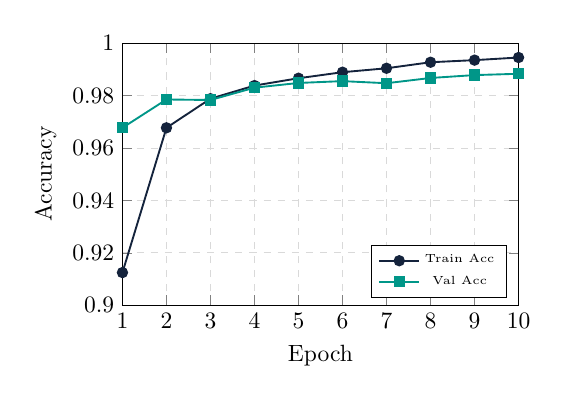
\begin{tikzpicture}[scale=0.85]
                \begin{axis}[
                    width=7.5cm, height=5.5cm,
                    xlabel={Epoch}, ylabel={Accuracy},
                    xmin=1, xmax=10, ymin=0.9, ymax=1.0,
                    xtick={1,2,3,4,5,6,7,8,9,10},
                    grid=both, grid style={dashed, gray!30},
                    legend pos=south east,
                    legend style={font=\tiny}
                ]
                \addplot[color=primary, mark=*, thick] coordinates {
                    (1, 0.9125) (2, 0.9677) (3, 0.9788) (4, 0.9838) (5, 0.9866) 
                    (6, 0.9889) (7, 0.9904) (8, 0.9927) (9, 0.9935) (10, 0.9945)
                };
                \addplot[color=secondary, mark=square*, thick] coordinates {
                    (1, 0.9677) (2, 0.9785) (3, 0.9783) (4, 0.9830) (5, 0.9848) 
                    (6, 0.9855) (7, 0.9847) (8, 0.9867) (9, 0.9878) (10, 0.9883)
                };
                \legend{Train Acc, Val Acc}
                \end{axis}
            \end{tikzpicture}
            \captionof{figure}{LeNet-5 Accuracy Curves over 10 Epochs}
        \end{column}
        \begin{column}{0.45\textwidth}
            \textbf{Dataset: MNIST Digit Classification}
            \begin{itemize}
                \item $60,000$ training images, $10,000$ testing.
                \item Normalization scaled inputs to $[0, 1]$.
            \end{itemize}
            \vspace{0.2cm}
            \textbf{Training Dynamics (10 Epochs):}
            \begin{itemize}
                \item \textbf{Rapid Learning:} Achieves $>96.7\%$ validation accuracy in just 1 epoch.
                \item \textbf{No Overfitting:} High validation generalization tracking training metrics perfectly.
                \item \textbf{Final Test Performance:}
                    \begin{itemize}
                        \item Test Loss: \textbf{0.0455}
                        \item Test Accuracy: \textbf{98.61\%}
                    \end{itemize}
            \end{itemize}
        \end{column}
    \end{columns}
\end{frame}

% ==================== Case Study 2: MobileNet-V2 Predecessor ====================
\begin{frame}{MobileNet-V2: Evolution from Predecessors}
    \begin{columns}
        \begin{column}{0.5\textwidth}
            \textbf{The Predecessor 1: Standard Convolutions}
            \begin{itemize}
                \item Extract spatial & channel information simultaneously.
                \item High parameter counts and multiplication complexity.
            \end{itemize}
            \vspace{0.2cm}
            \textbf{The Predecessor 2: MobileNet-V1 (2017)}
            \begin{itemize}
                \item Introduced \textbf{Depthwise Separable Convolutions}:
                \item Splits standard conv into:
                    \begin{enumerate}
                        \item \textbf{Depthwise (DW):} Scans spatially using 1 filter per input channel.
                        \item \textbf{Pointwise (PW):} $1\times1$ conv combining channel information.
                    \end{enumerate}
                \item Dramatically reduces computational complexity by $\approx 8\times$ to $9\times$ with minimal accuracy drop.
            \end{itemize}
        \end{column}
        \begin{column}{0.5\textwidth}
            \begin{block}{Innovations of MobileNet-V2 (2018)}
                Built on V1 but introduced two massive structural enhancements:
                \vspace{0.2cm}
                \begin{enumerate{}}
                    \item \textbf{Inverted Residual Blocks:}
                        \begin{itemize}
                            \item ResNet used thick-thin-thick residuals.
                            \item MobileNet-V2 uses thin-thick-thin residuals: expands low-dimensional channels first, applies DW, then projects back.
                        \end{itemize}
                    \item \textbf{Linear Bottlenecks:}
                        \begin{itemize}
                            \item Removes non-linear activations (ReLU) in the final $1\times1$ projection layer.
                            \item Non-linearities on low dimensions crush important feature information.
                        \end{itemize}
                \end{enumerate}
            \end{block}
        \end{column}
    \end{columns}
\end{frame}

% ==================== MobileNet-V2 Architecture Detail (TikZ) ====================
\begin{frame}{MobileNet-V2: Inside the Inverted Residual Block}
    \centering
    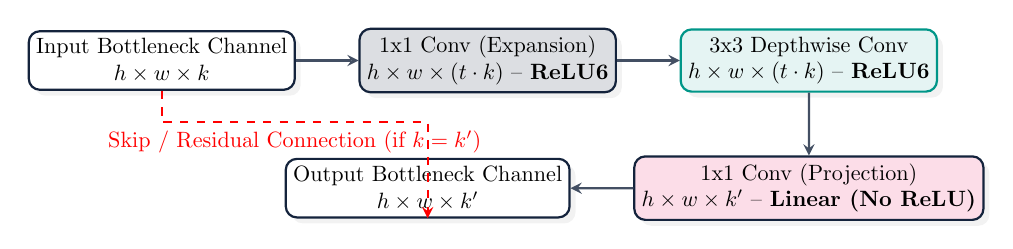
\begin{tikzpicture}[node distance=1.0cm, auto, scale=0.8, every node/.style={transform shape}]
        \node (in) [layer] {Input Bottleneck Channel\\$h \times w \times k$};
        \node (exp) [layer, fill=primary!15, right=of in] {1x1 Conv (Expansion)\\$h \times w \times (t \cdot k)$ -- \textbf{ReLU6}};
        \node (dw) [pool, right=of exp] {3x3 Depthwise Conv\\$h \times w \times (t \cdot k)$ -- \textbf{ReLU6}};
        \node (proj) [layer, fill=accent!15, below=1.0cm of dw] {1x1 Conv (Projection)\\$h \times w \times k'$ -- \textbf{Linear (No ReLU)}};
        \node (out) [layer, left=of proj] {Output Bottleneck Channel\\$h \times w \times k'$};
        
        \draw [arrow] (in) -- (exp);
        \draw [arrow] (exp) -- (dw);
        \draw [arrow] (dw) -- (proj);
        \draw [arrow] (proj) -- (out);
        
        % Skip Connection
        \path (in) -- (out) coordinate[midway] (mid);
        \draw [arrow, dashed, red] (in.south) -- ++(0,-0.5) -| node[pos=0.25, below] {Skip / Residual Connection (if $k = k'$)} (out.south);
    \end{tikzpicture}
    \vspace{0.4cm}
    \begin{itemize}
        \item \textbf{Expansion ($t$):} Expands channel space (typically $t=6$) to project spatial data into a high-dimensional manifold, making depthwise convolution much more effective.
        \item \textbf{Linear Bottleneck:} Keeps features clean by removing ReLU on the final low-dimensional projection.
    \end{itemize}
\end{frame}

% ==================== MobileNet-V2 Annotated Code ====================
\begin{frame}[fragile]{Annotated MobileNet-V2 Transfer Learning Code}
    \begin{lstlisting}[language=Python, caption={MobileNet-V2 Sequential wrapper for face anti-spoofing}]
# Load pre-trained MobileNetV2 base (built on ImageNet feature extractor)
base_model = applications.MobileNetV2(
    input_shape=(224, 224, 3), # Expected standard dimensions
    include_top=False,         # Discards original 1000-class classifier
    weights='imagenet'         # Uses pre-trained ImageNet parameters
)

# Freeze the backbone for high-efficiency feature extraction
base_model.trainable = False   # Keeps ImageNet representations frozen

# Custom Classification Head added sequentially
model = models.Sequential([
    base_model,                      # Pre-trained feature extractor base
    layers.GlobalAveragePooling2D(), # Spatial pooling reducing dimensions to 1280 nodes
    layers.Dropout(0.2),             # 20% Dropout to avoid overfitting in head
    layers.Dense(units=1, activation='sigmoid') # Sigmoid layer for binary classification
])

# Compiling model with learning rate suited for transfer learning head
model.compile(
    optimizer=optimizers.Adam(learning_rate=0.001),
    loss='binary_crossentropy',      # Ideal for Spoof/Real binary class
    metrics=['accuracy']
)
    \end{lstlisting}
\end{frame}

% ==================== MobileNet-V2 Dataset & Performance ====================
\begin{frame}{MobileNet-V2 Dataset & Performance Evaluation}
    \begin{columns}
        \begin{column}{0.55\textwidth}
            \centering
            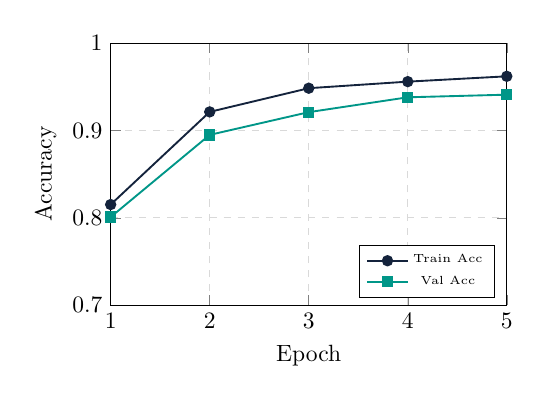
\begin{tikzpicture}[scale=0.85]
                \begin{axis}[
                    width=7.5cm, height=5.5cm,
                    xlabel={Epoch}, ylabel={Accuracy},
                    xmin=1, xmax=5, ymin=0.7, ymax=1.0,
                    xtick={1,2,3,4,5},
                    grid=both, grid style={dashed, gray!30},
                    legend pos=south east,
                    legend style={font=\tiny}
                ]
                \addplot[color=primary, mark=*, thick] coordinates {
                    (1, 0.8153) (2, 0.9213) (3, 0.9484) (4, 0.9559) (5, 0.9620)
                };
                \addplot[color=secondary, mark=square*, thick] coordinates {
                    (1, 0.8010) (2, 0.8950) (3, 0.9210) (4, 0.9380) (5, 0.9410)
                };
                \legend{Train Acc, Val Acc}
                \end{axis}
            \end{tikzpicture}
            \captionof{figure}{MobileNet-V2 Accuracy Curves over 5 Epochs}
        \end{column}
        \begin{column}{0.45\textwidth}
            \textbf{Dataset: Face Anti-Spoofing}
            \begin{itemize}
                \item Real Faces vs. Fake (Spoofed) Faces.
                \item $16,000$ training images, $4,000$ validation.
            \end{itemize}
            \vspace{0.2cm}
            \textbf{Training Performance Summary:}
            \begin{itemize}
                \item \textbf{Rapid Convergence:} Extremely fast training leveraging pre-trained ImageNet filters.
                \item \textbf{Excellent Generalization:}
                    \begin{itemize}
                        \item Final Training Accuracy: \textbf{96.20\%}
                        \item Final Validation Accuracy: \textbf{94.10\%}
                        \item Landmark performance: Achieves \textbf{almost 94\% (93.80\%)} accuracy on validation by epoch 4.
                    \end{itemize}
                \item \textbf{Efficiency:} MobileNet-V2 runs highly light-weight operations with superior classification power.
            \end{itemize}
        \end{column}
    \end{columns}
\end{frame}

% ==================== Transfer Learning Methodology ====================
\begin{frame}{Best Practices for Transfer Learning Success}
    \begin{block}{Why Transfer Learning Excels}
        Deep networks trained on huge datasets (ImageNet) have already learned generalized features (edges, contours, gradients). Transferring these pre-trained weights to face anti-spoofing saves massive computational hours and avoids overfitting on moderate-sized datasets.
    \end{block}
    \vspace{0.2cm}
    \begin{columns}
        \begin{column}{0.5\textwidth}
            \textbf{Phase 1: Feature Extraction (Frozen)}
            \begin{itemize}
                \item Set `base\_model.trainable = False`.
                \item Freeze pre-trained representations.
                \item Train only the custom Dense classification head.
                \item Highly computational-saving: $>90\%$ of network gradients are not calculated.
            \end{itemize}
        \end{column}
        \begin{column}{0.5\textwidth}
            \textbf{Phase 2: Fine-Tuning (Selective)}
            \begin{itemize}
                \item Unfreeze the top layers of MobileNet-V2.
                \item Recompile using a very small learning rate (e.g. $lr = 10^{-5}$).
                \item Adapts the deep convolutional filters to fine-grained face anti-spoofing features without destroying global knowledge.
            \end{itemize}
        \end{column}
    \end{columns}
\end{frame}

% ==================== Trade-off Analysis ====================
\begin{frame}{Computational Trade-off Analysis}
    \centering
    \small
    \begin{tabular}{lll}
        \toprule
        \textbf{Metric} & \textbf{LeNet-5 (Digit Recognizer)} & \textbf{MobileNet-V2 (Anti-Spoofing)} \\
        \midrule
        \textbf{Primary Design Focus} & Simple handwritten digit classification & Lightweight efficiency for portable/edge devices \\
        \textbf{Key Innovations} & Spatial weight sharing, local pooling & Inverted residuals, linear bottlenecks \\
        \textbf{Dataset Implemented} & MNIST ($32\times32$ padded) & Custom Face Dataset ($224\times224\times3$ augmented) \\
        \textbf{Total Parameters} & \textbf{61,706} & \textbf{2,257,985} \\
        \textbf{Computational Cost} & Low (negligible FLOPS) & Extremely low for deep nets (300M MAdds) \\
        \textbf{Hardware Target} & Standard CPU & Mobile / Edge CPUs / low-power GPUs \\
        \textbf{Training Method} & Standard Train from Scratch & Transfer Learning (Base Frozen + Head Trained) \\
        \textbf{Best Validation Accuracy} & \textbf{98.83\%} & \textbf{94.10\%} (Almost 94\% at Epoch 4) \\
        \bottomrule
    \end{tabular}
    \normalsize
    \vspace{0.4cm}
    \begin{itemize}
        \item \textbf{Conclusion 1:} Custom shallow networks (LeNet-5) are efficient & robust for low-resolution tasks.
        \item \textbf{Conclusion 2:} High-dimensional transfer learning (MobileNet-V2) yields world-class performance, but requires proper layer freezing to avoid catastrophic forgetting and severe overfitting.
    \end{itemize}
\end{frame}

% ==================== Summary ====================
\begin{frame}{Assignment Summary & Takeaways}
    \begin{itemize}
        \item \textbf{Evolutionary Path:} CNN design has shifted from simply adding layers (which leads to extreme parameters) to designing smart structural blocks (inverted residuals, depthwise separability) to maximize accuracy-per-parameter.
        \item \textbf{LeNet-5 Significance:} Proved that automatic parameter-shared spatial scanning crushes manual feature engineering.
        \item \textbf{MobileNet-V2 Power:} Delivers deep modern representational capacity at a fraction of the computational and memory footprint of ResNet or VGG.
        \item \textbf{Practical Engineering Lesson:} Deep learning pipelines are highly sensitive to configuration details (unfrozen layers, learning rates, target tasks). Model architectures are only as strong as their training hygiene.
    \end{itemize}
    \vspace{0.4cm}
    \centering
    \large\color{primary}\textbf{Thank You! Questions?}
\end{frame}

\end{document}
